%%% DOCUMENTCLASS 
%%%-------------------------------------------------------------------------------

\documentclass[
a4paper, % Stock and paper size.
11pt, % Type size.
% article,
% oneside, 
onecolumn, % Only one column of text on a page.
% openright, % Each chapter will start on a recto page.
% openleft, % Each chapter will start on a verso page.
openany, % A chapter may start on either a recto or verso page.
]{memoir}

%%% PACKAGES 
%%%------------------------------------------------------------------------------

\usepackage[utf8]{inputenc} % If utf8 encoding
% \usepackage[lantin1]{inputenc} % If not utf8 encoding, then this is probably the way to go
\usepackage[T1]{fontenc}    %
\usepackage{lmodern}
\usepackage[english]{babel} % English please
\usepackage[final]{microtype} % Less badboxes

% \usepackage{kpfonts} %Font

\usepackage{amsmath,amssymb,mathtools} % Math

% \usepackage{tikz} % Figures
\usepackage{graphicx} % Include figures
\usepackage{makeidx}

%%% PAGE LAYOUT 
%%%-----------------------------------------------------------------------------
\setlrmarginsandblock{0.15\paperwidth}{*}{1} % Left and right margin
\setulmarginsandblock{0.2\paperwidth}{*}{1}  % Upper and lower margin
\checkandfixthelayout

\newlength\forceindent
\setlength{\forceindent}{\parindent}
\setlength{\parindent}{0cm}
\renewcommand{\indent}{\hspace*{\forceindent}}
\setlength{\parskip}{1em}


%%% SECTIONAL DIVISIONS
%%%------------------------------------------------------------------------------

\maxsecnumdepth{subsection} % Subsections (and higher) are numbered
\setsecnumdepth{subsection}

\makeatletter %
\makechapterstyle{standard}{
  \setlength{\beforechapskip}{0\baselineskip}
  \setlength{\midchapskip}{1\baselineskip}
  \setlength{\afterchapskip}{8\baselineskip}
  \renewcommand{\chapterheadstart}{\vspace*{\beforechapskip}}
  \renewcommand{\chapnamefont}{\centering\normalfont\Large}
  \renewcommand{\printchaptername}{\chapnamefont \@chapapp}
  \renewcommand{\chapternamenum}{\space}
  \renewcommand{\chapnumfont}{\normalfont\Large}
  \renewcommand{\printchapternum}{\chapnumfont \thechapter}
  \renewcommand{\afterchapternum}{\par\nobreak\vskip \midchapskip}
  \renewcommand{\printchapternonum}{\vspace*{\midchapskip}\vspace*{5mm}}
  \renewcommand{\chaptitlefont}{\centering\bfseries\LARGE}
%  \renewcommand{\printchaptertitle}[1]{\chaptitlefont ##1}
  \renewcommand{\afterchaptertitle}{\par\nobreak\vskip \afterchapskip}
}
\makeatother

%\chapterstyle{standard}
\chapterstyle{madsen}

\setsecheadstyle{\normalfont\large\bfseries}
\setsubsecheadstyle{\normalfont\normalsize\bfseries}
\setparaheadstyle{\normalfont\normalsize\bfseries}
\setparaindent{0pt}\setafterparaskip{0pt}

%%% FLOATS AND CAPTIONS
%%%------------------------------------------------------------------------------

\makeatletter                  % You do not need to write [htpb] all the time
\renewcommand\fps@figure{htbp} %
\renewcommand\fps@table{htbp}  %
\makeatother                   %

\captiondelim{\space } % A space between caption name and text
\captionnamefont{\small\bfseries} % Font of the caption name
\captiontitlefont{\small\normalfont} % Font of the caption text

\changecaptionwidth          % Change the width of the caption
\captionwidth{1\textwidth} %

%%% ABSTRACT
%%%------------------------------------------------------------------------------

\renewcommand{\abstractnamefont}{\normalfont\small\bfseries} % Font of abstract title
\setlength{\absleftindent}{0.1\textwidth} % Width of abstract
\setlength{\absrightindent}{\absleftindent}

%%% HEADER AND FOOTER 
%%%------------------------------------------------------------------------------

\makepagestyle{standard} % Make standard pagestyle

\makeatletter                 % Define standard pagestyle
\makeevenfoot{standard}{}{}{} %
\makeoddfoot{standard}{}{}{}  %
\makeevenhead{standard}{\bfseries\thepage\normalfont\qquad\small\leftmark}{}{}
\makeoddhead{standard}{}{}{\small\rightmark\qquad\bfseries\thepage}
% \makeheadrule{standard}{\textwidth}{\normalrulethickness}
\makeatother                  %

\makeatletter
\makepsmarks{standard}{
\createmark{chapter}{both}{shownumber}{\@chapapp\ }{ \quad }
\createmark{section}{right}{shownumber}{}{ \quad }
\createplainmark{toc}{both}{\contentsname}
\createplainmark{lof}{both}{\listfigurename}
\createplainmark{lot}{both}{\listtablename}
\createplainmark{bib}{both}{\bibname}
\createplainmark{index}{both}{\indexname}
\createplainmark{glossary}{both}{\glossaryname}
}
\makeatother                               %

\makepagestyle{chap} % Make new chapter pagestyle

\makeatletter
\makeevenfoot{chap}{}{\small\bfseries\thepage}{} % Define new chapter pagestyle
\makeoddfoot{chap}{}{\small\bfseries\thepage}{}  %
\makeevenhead{chap}{}{}{}   %
\makeoddhead{chap}{}{}{}    %
% \makeheadrule{chap}{\textwidth}{\normalrulethickness}
\makeatother

\nouppercaseheads
\pagestyle{standard}               % Choosing pagestyle and chapter pagestyle
\aliaspagestyle{chapter}{chap} %


%%% NEW COMMANDS
%%%-----------------------------------------------------------------------------


\newcommand{\p}{\partial} %Partial
% Or what ever you want


%%% CODE SNIPPETS, COMMANDS, ETC
%%%-----------------------------------------------------------------------------
\usepackage{xcolor}
\usepackage{listings} % Display code / shell commands
%\newcommand{\shellcommand}[1]{\begin{lstlisting} \#1 \end{lstlisting}
\lstdefinestyle{BashInputStyle}{
  language=bash,
  basicstyle=\small\sffamily,
%  numbers=left,
%  numberstyle=\tiny,
%  numbersep=3pt,
  frame=,
  columns=fullflexible,
  backgroundcolor=\color{black!05},
  linewidth=0.9\linewidth,
  xleftmargin=0.1\linewidth
}
\definecolor{gray}{rgb}{0.4,0.4,0.4}
\definecolor{darkblue}{rgb}{0.0,0.0,0.6}
\definecolor{cyan}{rgb}{0.0,0.6,0.6}
\definecolor{maroon}{rgb}{0.5,0.0,0.0}
\lstdefinelanguage{XML}
{
  basicstyle=\ttfamily\footnotesize,
  morestring=[b]",
  moredelim=[s][\bfseries\color{maroon}]{<}{\ },
  moredelim=[s][\bfseries\color{maroon}]{</}{>},
  moredelim=[l][\bfseries\color{maroon}]{/>},
  moredelim=[l][\bfseries\color{maroon}]{>},
  morecomment=[s]{<?}{?>},
  morecomment=[s]{<!--}{-->},
  commentstyle=\color{gray},
  stringstyle=\color{orange},
  identifierstyle=\color{darkblue}
}
\lstdefinestyle{XMLStyle}{
  language=XML,
  basicstyle=\sffamily\footnotesize,
  numbers=left,
  numberstyle=\tiny,
  numbersep=3pt,
  frame=,
  columns=fullflexible,
  backgroundcolor=\color{black!05},
  linewidth=0.9\linewidth,
  xleftmargin=0.1\linewidth
}


%%% TABLE OF CONTENTS AND INDEX
%%%-----------------------------------------------------------------------------

\maxtocdepth{subsection} % Only parts, chapters and sections in the table of contents
\settocdepth{subsection}

\makeindex

%\AtEndDocument{\addtocontents{toc}{\par}} % Add a \par to the end of the TOC

%%% INTERNAL HYPERLINKS
%%%-----------------------------------------------------------------------------
\usepackage[linktoc=all]{hyperref}   % Internal hyperlinks
\hypersetup{
colorlinks,
citecolor=darkblue,
filecolor=darkblue,
linkcolor=darkblue,
urlcolor=darkblue
pdfborder={0 0 0},      % No borders around internal hyperlinks
pdfauthor={I am the Author} % author
}
\usepackage{memhfixc}   %


%%% PRETTY TITLE PAGE FOR PDF DOC
%%%-----------------------------------------------------------------------------
\makeatletter
\newlength\drop
\newcommand{\br}{\hfill\break}
\newcommand*{\titlepage}{%
    \thispagestyle{empty}
    \begingroup% Gentle Madness
    \drop = 0.1\textheight
    \vspace*{\baselineskip}
    \vfill
    \hbox{%
      \hspace*{0.1\textwidth}%
      \rule{1pt}{\dimexpr\textheight-28pt\relax}%
      \hspace*{0.05\textwidth}% 
      \parbox[b]{0.85\textwidth}{%
        \vbox{%
          \vspace{\drop}
          {\Huge\bfseries\raggedright\@title\par}
          \vskip2.37\baselineskip
          {\huge\bfseries Version \input{../../VERSION}\par}
          \vskip4\baselineskip
          {\huge\bfseries \textcolor{darkblue}{Developer Guide}\par}
          \vskip1.0\baselineskip
          {\large\bfseries\@date\par}
          \vspace{0.3\textheight}
          {\small\noindent\@author}\\[\baselineskip]
        }% end of vbox
      }% end of parbox
    }% end of hbox
    \vfill
    \null
\endgroup}
\makeatother

%%% THE DOCUMENT
%%% Where all the important stuff is included!
%%%-------------------------------------------------------------------------------

\author{Department of Aeronautics, Imperial College London, UK\\
Scientific Computing and Imaging Institute, University of Utah, USA}
\title{Nektar++: Spectral/hp Element Framework}
\date{\today}

\begin{document}

\frontmatter

% Render pretty title page if not building HTML
\ifdefined\HCode
\maketitle
\else
\titlepage
\fi

\clearpage

\ifx\HCode\undefined
\tableofcontents*
\fi

\clearpage

\chapter{Introduction}
Welcome to the developer's guide for Nektar++\cite{nektar-website}.

\mainmatter

\chapter{Core Concepts}

This section describes some of the key concepts which are useful when developing
code within the Nektar++ framework.

\section{Factory method pattern}
The factory method pattern is used extensively throughout Nektar++ as a
mechanism to instantiate objects. It provides the following benefits:
\begin{itemize}
\item Encourages modularisation of code such that conceptually related
algorithms are grouped together
\item Structuring of code such that different implementations of the same
concept are encapsulated and share a common interface
\item Users of a factory-instantiated modules need only be concerned with the
 interface and not the details of underlying implementations
\item Simplifies debugging since code relating to a specific implementation
 resides in a single class
\item The code is naturally decoupled to reduce header-file dependencies and
 improves compile times
\item Enables implementations (e.g. relating to third-party libraries) to be
 disabled through the build process (CMake) by not compiling a specific 
 implementation, rather than scattering preprocessing statements throughout the
 code
\end{itemize}

For conceptual details see the Wikipedia page.
%\url{http://en.wikipedia.org/wiki/Factory_pattern}.

\subsection{Using NekFactory}
The templated NekFactory class implements the factory pattern in Nektar++.
There are two distinct aspects to creating a factory-instantiated collection of
classes: defining the public interface, and registering specific
implementations. Both of these involve adding standard boilerplate code. It is
assumed that we are writing a code which implements a particular concept or
functionality within the code, for which there are multiple implementations. The
reasons for multiple implementations may be very low level such as alternative
algorithms for solving a linear system, or high level, such as selecting from a
range of PDEs to solve.

\subsubsection{Creating an interface (base class)}
A base class must be defined which prescribes an implementation-independent
interface. In Nektar++, the template method pattern is used, requiring public
interface functions to be defined which call private virtual implementation
methods. The latter will be overridden in the specific implementation classes.
In the base class these virtual methods should be defined as pure virtual, since
there is no implementation and we will not be instantiating this base class
explicitly.

As an example we will create a factory for instantiating different
implementations of some concept \inlsh{MyConcept}, defined in
\inlsh{MyConcept.h} and \inlsh{MyConcept.cpp}. First in \inlsh{MyConcept.h},
we need to include the NekFactory header

\begin{lstlisting}[style=C++Style]
#include <LibUtilities/BasicUtils/NekFactory.hpp>
\end{lstlisting}

The following code should then be included just before the base class
declaration (in the same namespace as the class):

\begin{lstlisting}[style=C++Style]
class MyConcept

// Datatype for the MyConcept factory
typedef LibUtilities::NekFactory< std::string, MyConcept, 
            ParamType1,
            ParamType2 > MyConceptFactory;
MyConceptFactory& GetMyConceptFactory();
\end{lstlisting}

The template parameters define the datatype of the key used to retrieve a
particular implementation (usually a string, enum or custom class such as
\inlsh{MyConceptKey}, the base class (in our case \inlsh{MyConcept} and a list
of zero or more parameters which are taken by the constructors of all
implementations of the type \inlsh{MyConcept} (in our case we have two). Note
that all implementations must take the same parameter list in their constructors.

The normal definition of our base class then follows:

\begin{lstlisting}[style=C++Style]
class MyConcept 
{
    public:
        MyConcept(ParamType1 p1, ParamType2 p2);
        ...
};
\end{lstlisting}

We must also define a shared pointer for our base class for use later
\begin{lstlisting}[style=C++Style]
typedef boost::shared_ptr<MyConcept> MyConceptShPtr;
\end{lstlisting}

\subsubsection{Creating a specific implementation (derived class)}
A class is defined for each specific implementation of a concept. It is these
specific implementations which are instantiated by the factory.

In our example we will have an implementations called \inlsh{MyConceptImpl1}
defined in \inlsh{MyConceptImpl1.h} and \inlsh{MyConceptImpl1.cpp}. In the
header file we include the base class header file

\begin{lstlisting}[style=C++Style]
#include <Subdir/MyConcept.h>
\end{lstlisting}

We then define the derived class as normal:

\begin{lstlisting}[style=C++Style]
class MyConceptImpl1 : public MyConcept
{
...
};
\end{lstlisting}

In order for the factory to work, it must know
\begin{itemize}
\item that {{{MyConceptImpl1}}} exists, and
\item how to create it.
\end{itemize}

To allow the factory to create instances of our class we define a function in 
our class:
\begin{lstlisting}[style=C++Style]
/// Creates an instance of this class
static MyConceptSharedPtr create(
            ParamType1 p1,
            ParamType2 p2)
{
    return MemoryManager<MyConceptImpl1>::AllocateSharedPtr(p1, p2);
}
\end{lstlisting}
This function simply creates an instance of \inlsh{MyConceptImpl1} using the
supplied parameters. It must be \inlsh{static} because we are not operating on
an existing instance and it should return a base class shared pointer (rather 
than a \inlsh{MyConceptImpl1} shared pointer), since the point of the factory
is that the calling code does not know about specific implementations.

The last task is to register our implementation with the factory. This is done 
using the \inlsh{RegisterCreatorFunction} member function of the factory.
However, we wish this to happen as early on as possible (so we can use the 
factory straight away) and without needing to explicitly call the function for 
every implementation at the beginning of our program (since this would again 
defeat the point of a factory)! The solution is to use the function to 
initialise a static variable: it will be executed prior to the start of the
\inlsh{main()} routine, and can be located within the very class it is
registering, satisfying our code decoupling requirements.

In \inlsh{MyConceptImpl1.h} we define a static variable with the same datatype
as the key used in our factory (in our case \inlsh{std::string}) 
\begin{lstlisting}[style=C++Style]
static std::string className;
\end{lstlisting}
The above variable can be \inlsh{private} since it is typically never actually
used within the code. We then initialise it in \inlsh{MyConceptImpl1.cpp}

\begin{lstlisting}[style=C++Style] 
string MyConceptImpl1::className
        = GetMyConceptFactory().RegisterCreatorFunction(
            "Impl1", MyConceptImpl1::create, "First implementation of my
            concept.");
\end{lstlisting}
The first parameter specifies the value of the key which should be used to
select this implementation. The second parameter is a function pointer to our
static function used to instantiate our class. The third parameter provides a
description which can be printed when listing the available MyConcept
implementations.

\subsection{Instantiating classes}
To create instances of MyConcept implementations elsewhere in the code, we must
first include the ''base class'' header file
\begin{lstlisting}[style=C++Style]
#include <Subdir/MyConcept.h>
\end{lstlisting}
Note we do not include the header files for the specific MyConcept 
implementations anywhere in the code (apart from \inlsh{MyConceptImpl1.cpp}).
If we modify the implementation, only the implementation itself requires 
recompiling and the executable relinking.

We create an instance by retrieving the \inlsh{MyConceptFactory} and call the
\inlsh{CreateInstance} member function of the factory:
\begin{lstlisting}[style=C++Style]
ParamType p1 = ...;
ParamType p2 = ...;
MyConceptShPtr p = GetMyConceptFactory().CreateInstance( "Impl1", p1, p2 );
\end{lstlisting}

Note that the class is used through the pointer \inlsh{p}, which is of type
\inlsh{MyConceptShPtr}, allowing the use of any of the public interface
functions in the base class (and therefore the specific implementations behind them) to be
called, but not directly any functions declared solely in a specific
implementation.


\chapter{Library Design}

A major challenge which arises when one aims to develop a software package that
implements the spectral/hp element method is to implement the mathematical
structure of the method in a digestible and coherent matter. Obviously, there
are many ways to encapsulate the fundamental concepts related to the
spectral/$hp$ element method, depending on e.g. the intended goal of the
developer or the chosen programming language. We will (without going in too much
detail) give a an overview of how we have chosen to abstract and implement
spectral/hp elements in the \nekpp library. However, we want to emphasise that
this is not the only possible choice.

Five different sublibraries, employing this characteristic pattern, are provided
in the full \nekpp library:

\begin{itemize}
\item the supporting utilities sublibrary (LibUtilities library)
\item the standard elemental region sublibrary (StdRegions library)
\item the parametric mapping sublibrary (SpatialDomains library)
\item the local elemental region sublibrary (LocalRegions library)
\item the global region sublibrary (MultiRegions library)
\item the solver support sublibrary (SolverUtils library)
\end{itemize}

This structure can also be related to the formulation of a global spectral/hp
element expansion, i.e.

\begin{align*}
  u(\boldsymbol{x})=\overbrace{\sum_{e\in\mathcal{E}}\underbrace{\sum_{n\in\mathcal{N}}\phi^e_n(\boldsymbol{x})\hat{u}^e_n}_{\mbox{\scriptsize{LocalRegions
  library}}}}^{\mbox{\scriptsize{MultiRegions
  library}}}=\sum_{e\in\mathcal{E}}\underbrace{\sum_{n\in\mathcal{N}}\phi^{std}_n\overbrace{(\left[\chi^e\right]^{-1}(\boldsymbol{x}))}^{\mbox{\scriptsize{SpatialDomains
  library}}}\hat{u}^e_n}_{\mbox{\scriptsize{StdRegions library}}}
\end{align*}

A more detailed overview of the \nekpp structure is given in
Figure~\ref{f:library:structure}. A diagram showing the most important classes
in the core sub-libraries, is depicted in the Figure~\ref{f:library:overview}.

\begin{figure}
\centering
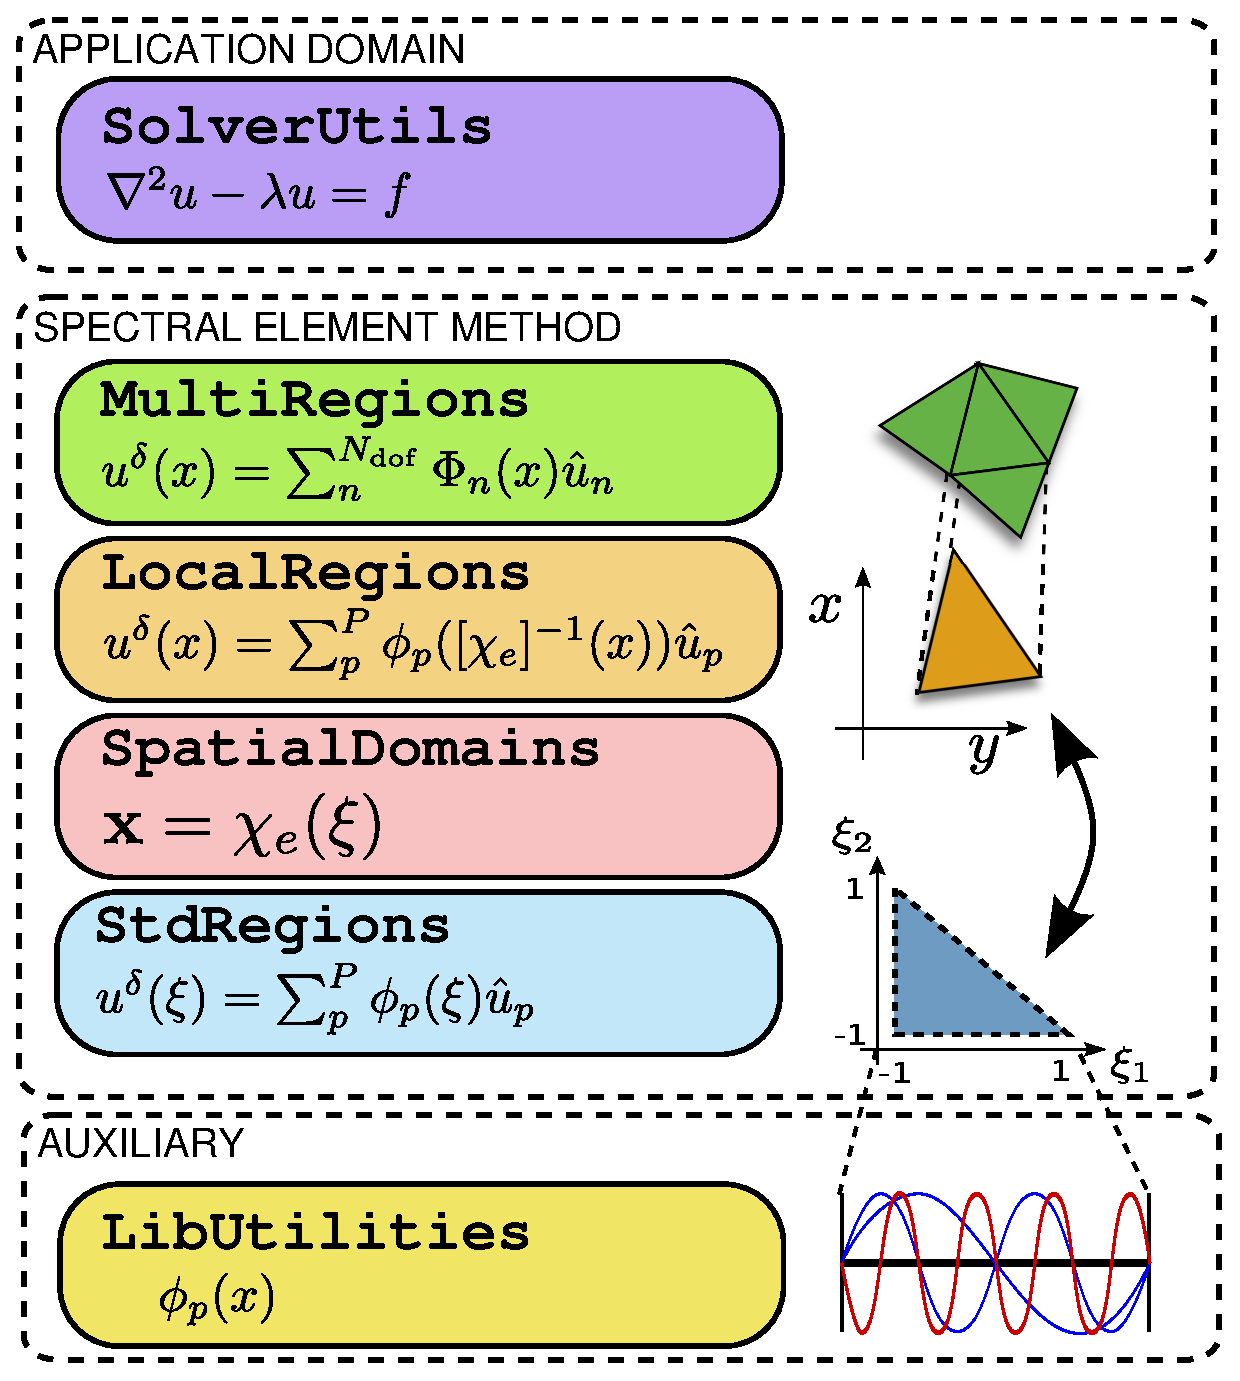
\includegraphics[width=0.6\textwidth]{img/architecture}
\caption{Structural overview of the Nektar++ libraries}
\label{f:library:structure}
\end{figure}

\begin{figure}
\centering
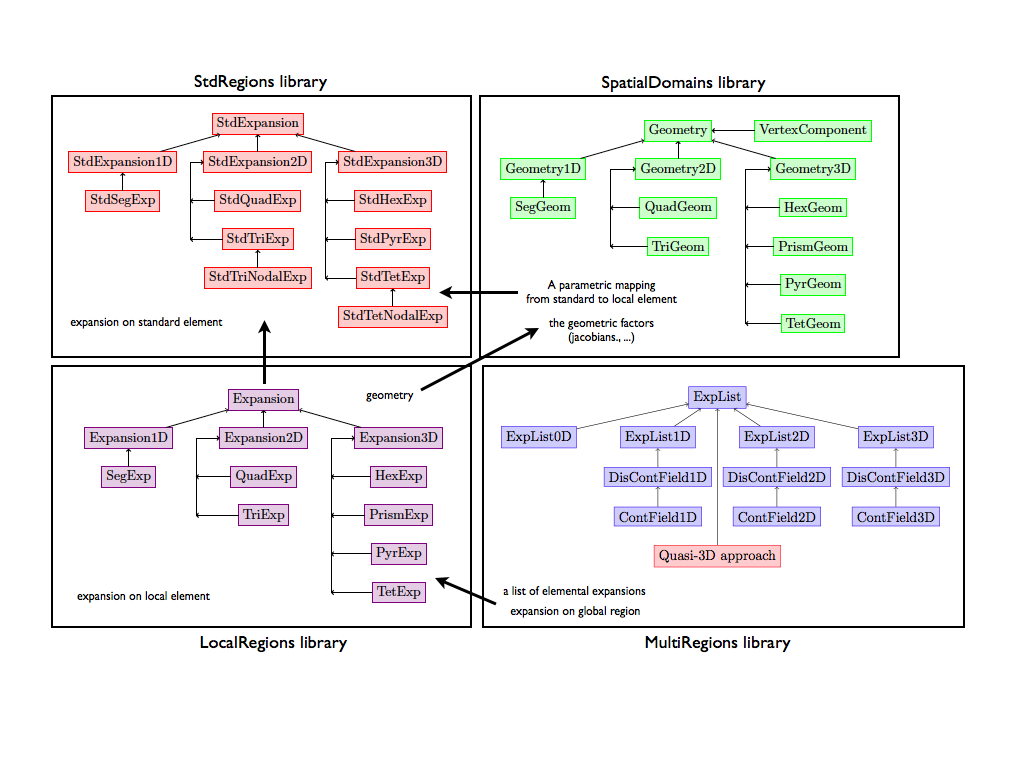
\includegraphics[width=\textwidth]{img/overview.png}
\caption{Diagram of the important classes in each library.}
\label{f:library:overview}
\end{figure}

\section{LibUtilities}

This contains the underlying building blocks for constructing a spectral element
formulation including linear algebra, polynomial routines and memory management
\cite{Ga39,AbSt64,CaHuYoQu88,GhOs70,KaSh05}. This includes:
\begin{itemize}
\setlength{\itemsep}{0em}
\item Basic Constants
\item Basic Utilities ( Nektar++ Arrays)
\item Expression Templates
\item Foundations
\item Interpreter
\item Kernel
\item Linear Algebra
\item Memory Management
\item Nodal Data
\item Polynomial Subroutines
\item Time Integration
\end{itemize}

\subsection{The Polylib library}
These are routines for orthogonal polynomial calculus and interpolation based on
codes by Einar Ronquist and Ron Henderson.

\subsubsection{Abbreviations}
\begin{tabular}{ll}
\toprule
Character(s) & Description \\
\midrule
z & Set of collocation/quadrature points \\
w & Set of quadrature weights \\
D & Derivative matrix \\
h & Lagrange Interpolant \\
I & Interpolation matrix \\
g & Gauss \\
k & Kronrod \\
gr & Gauss-Radau \\
gl & Gauss-Lobatto \\
j & Jacobi \\
m & point at minus 1 in Radau rules \\
p & point at plus 1 in Radau rules \\
\bottomrule
\end{tabular}


\subsubsection{Main routines}
\begin{tabular}{ll}
\toprule
\multicolumn{2}{l}{\textbf{Points and Weights}} \\
Routine & Description \\
\midrule
zwgj & Compute Gauss-Jacobi points and weights \\
zwgrjm & Compute Gauss-Radau-Jacobi points and weights (z=-1) \\
zwgrjp & Compute Gauss-Radau-Jacobi points and weights (z= 1) \\
zwglj & Compute Gauss-Lobatto-Jacobi points and weights \\
zwgk & Compute Gauss-Kronrod-Jacobi points and weights \\
zwrk & Compute Radau-Kronrod points and weights \\
zwlk & Compute Lobatto-Kronrod points and weights \\
JacZeros & Compute Gauss-Jacobi points and weights \\
\bottomrule
\end{tabular}

\begin{tabular}{ll}
\toprule
\multicolumn{2}{l}{\textbf{Derivative Matrices}} \\
Routine & Description \\
\midrule
Dgj & Compute Gauss-Jacobi derivative matrix \\
Dgrjm & Compute Gauss-Radau-Jacobi derivative matrix (z=-1) \\
Dgrjp & Compute Gauss-Radau-Jacobi derivative matrix (z= 1) \\
Dglj & Compute Gauss-Lobatto-Jacobi derivative matrix \\
\bottomrule
\end{tabular}

\begin{tabular}{ll}
\toprule
\multicolumn{2}{l}{\textbf{Lagrange Interpolants}} \\
Routine & Description \\
\midrule
hgj & Compute Gauss-Jacobi Lagrange interpolants \\
hgrjm & Compute Gauss-Radau-Jacobi Lagrange interpolants (z=-1) \\
hgrjp & Compute Gauss-Radau-Jacobi Lagrange interpolants (z= 1) \\
hglj & Compute Gauss-Lobatto-Jacobi Lagrange interpolants \\
\bottomrule
\end{tabular}

\begin{tabular}{ll}
\toprule
\multicolumn{2}{l}{\textbf{Interpolation Operators}} \\
Routine & Description \\
\midrule
Imgj & Compute interpolation operator gj->m \\
Imgrjm & Compute interpolation operator grj->m (z=-1) \\
Imgrjp & Compute interpolation operator grj->m (z= 1) \\
Imglj & Compute interpolation operator glj->m \\
\bottomrule
\end{tabular}

\begin{tabular}{ll}
\toprule
\multicolumn{2}{l}{\textbf{Polynomial Evaluation}} \\
Routine & Description \\
\midrule
jacobfd & Returns value and derivative of Jacobi poly. at point z \\
jacobd & Returns derivative of Jacobi poly. at point z (valid at z=-1,1) \\
\bottomrule
\end{tabular}

\subsubsection{Local routines}
\begin{tabular}{ll}
\toprule
Routine & Description \\
\midrule
jacobz & Returns Jacobi polynomial zeros \\
gammaf & Gamma function for integer values and halves \\
RecCoeff & Calculates the recurrence coefficients for orthogonal poly \\
TriQL & QL algorithm for symmetrix tridiagonal matrix \\
JKMatrix & Generates the Jacobi-Kronrod matrix \\
\bottomrule
\end{tabular}

\subsubsection{Notes}
\begin{itemize}
\setlength{\itemsep}{0em}
\item Legendre polynomial $\alpha = \beta = 0$
\item Chebychev polynomial $\alpha = \beta = -0.5$
\item All routines are double precision.
\item All array subscripts start from zero, i.e. vector $0..N-1$
\end{itemize}



\section{StdRegions}
The StdRegions library, a summary of which is shown in
Figure~\ref{f:library:stdregions}, bundles all classes that mimic a
spectral/$hp$ element expansion on a standard region. Such an expansion, i.e.
\begin{align*}
u(\boldsymbol{\xi}_i) =
  \sum_{n\in\mathcal{N}}\phi_n(\boldsymbol{\xi}_i)\hat{u}_n,
\end{align*}
can be encapsulated in a class that essentially should only contain three data
structures, respectively representing:

\begin{itemize}
\item the coefficient vector $\hat{\boldsymbol{u}}$,
\item the discrete basis matrix $\boldsymbol{B}$, and
\item the vector $\boldsymbol{u}$ which represents the value of the expansion
at the quadrature points $\boldsymbol{\xi}_i$.
\end{itemize}

All standard expansions, independent of the dimensionality or shape of the
standard region, can be abstracted in a similar way. Therefore, it is possible
to define these data structures in an \emph{abstract} base class, i.e. the class
!StdExpansion. This base class can also contain the implementation of methods
that are identical across all shapes. Derived from this base class is another
level of abstraction, i.e. the abstract classes StdExpansion1D, StdExpansion2D
and StdExpansion3D. All other shape-specific classes (such as e.g. StdSegExp or
StdQuadExp) are inherited from these abstract base classes. These shape-specific
classes are the classes from which objects will be instantiated.
They also contain the shape-specific implementation for operations such as
integration or differentiation.

\begin{figure}
\centering
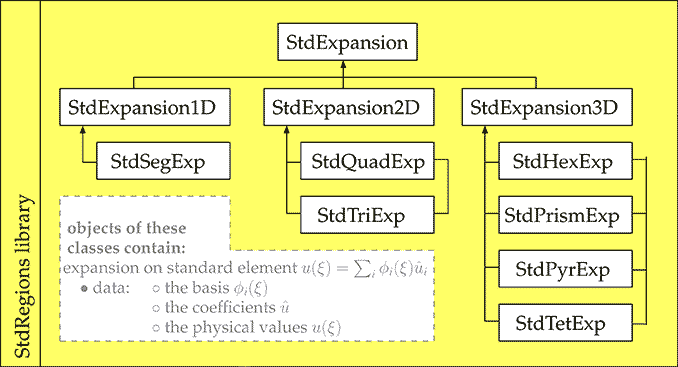
\includegraphics[width=\textwidth]{img/StdRegions.png}
\caption{Main classes in the StdRegions library.}
\label{f:library:stdregions}
\end{figure}

\section{SpatialDomains}
The most important family of classes in the SpatialDomains library is the
Geometry family, as can also be seen in Figure~\ref{f:library:spatialdomains}.
These classes are the representation of a (geometric) element in \emph{physical
space}. It has been indicated before that every local element can be considered
as an image of the standard element where the corresponding one-to-one mapping
can be represented as an elemental standard spectral/hp expansion. As such, a
proper encapsulation should at least contain data structures that represent such
an expansion in order to completely define the geometry of the element.
Therefore, we have equipped the classes in the Geometry family with the
following data structures:

\begin{itemize}
\item an object of !StdExpansion class, and
\item a data structure that contains the metric terms (Jacobian, derivative
  metrics) of the transformation.
\end{itemize}

Note that although the latter data structure is not necessary to define the 
geometry, it contains information inherent to the iso-parametric representation
of the element that can later be used in e.g. the LocalRegions library. Again,
the StdExpansion object can be defined in the abstract base class Geometry. 
However, for every shape-specific geometry class, it needs to be initialised 
according to the corresponding StdRegions class (e.g. for the QuadGeom class, 
it needs to be initialised as an StdQuadExp object).

\begin{figure}
\centering
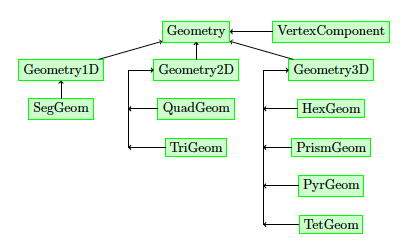
\includegraphics{img/SpatialDomains.png}
\caption{Main classes in the SpatialDomains library.}
\label{f:library:spatialdomains}
\end{figure}


\section{LocalRegions}
The LocalRegions library is designed to encompass all classes that encapsulate
the elemental spectral/hp expansions in physical space, see also the figure
below. It can be appreciated that such a local expansion essentially is a
standard expansion that has a (in C++ parlance) additional coordinate
transformation that maps the standard element to the local element. In an
object-oriented context, these is-a and has-a relationships can be applied as
follows: the classes in the !LocalRegions library are derived from the
{!StdExpansion} class tree but they are supplied with an additional data member
representing the geometry of the local element. Depending on the shape-specific
class in the !LocalRegions library, this additional data member is an object of
the corresponding class in the Geometry class structure. This inheritance
between the !LocalRegions and !StdRegions library also allows for a localised
implementation that prevents code duplication. In order to e.g. evaluate the
integral over a local element, the integrand can be multiplied by the Jacobian
of the coordinate transformation, where after the evaluation is redirected to
the !StdRegions implementation.

This provides extensions of the spectral element formulation into the world. It
provides spatially local forms of the reference space expansions through a
one-to-one linear mapping from a standard straight-sided region to the physical
space, based on the vertices.

\subsection{Local Mappings}

\subsubsection{Linear Mappings}
In one dimension this has the form
\begin{align*}
x = \chi(\xi) = \frac{1-\xi}{2}x_{e-1} + \frac{1+\xi}{2}x_e \quad \xi
\Omega^e
\end{align*}

In two dimensions, for a quadrilateral, each coordinate is given by
\begin{align*}
x_i = \chi(\xi_1,\xi_2) &= x_i^A\frac{1-\xi_1}{2}\frac{1-\xi_2}{2} +
x_i^B\frac{1+\xi_1}{2}\frac{1-\xi_2}{2} \\ &\qquad+
x_i^D\frac{1-\xi_1}{2}\frac{1+\xi_2}{2} +
x_i^C\frac{1+\xi_1}{2}\frac{1+\xi_2}{2}, \quad i=1,2
\end{align*}

\subsubsection{Curvilinear mappings}

The mapping can be extended to curved-sided regions through the use of an
iso-parametric representation. In contrast to the linear mapping, where only
information about the vertices of the element were required, a curvilinear
mapping requires information about the shape of each side. This is provided by
shape functions, $f^A(\xi_1), f^B(\xi_2), f^C(\xi_1)$ and
$f^D(\xi_2)$, in the local coordinate system. For example, the linear
blending function is given by
\begin{align*}
  x_i = \chi_i(\xi_1,\xi_2) &= f^A(\xi_1)\frac{1-\xi_2}{2} +
  f^C(\xi_1)\frac{1+\xi_2}{2} + f^B(\xi_2)\frac{1-\xi_1}{2} +
  f^D(\xi_2)\frac{1+\xi_1}{2}\\ &\qquad-
  \frac{1-\xi_1}{2}\frac{1-\xi_2}{2}f^A(-1) - 
  \frac{1+\xi_1}{2}\frac{1-\xi_2}{2}f^A(1)\\ &\qquad-
  \frac{1-\xi_1}{2}\frac{1+\xi_2}{2}f^C(-1) -
  \frac{1+\xi_1}{2}\frac{1+\xi_2}{2}f^C(1)
\end{align*}

\subsection{Classes}
All local expansions are derived from the top level Expansion base class. Three
classes, Expansion1D, Expansion2D and Expansion3D, are derived from this and
provided base classes for expansions in one-, two- and three- dimensions,
respectively. The various local expansions are derived from these. The class
hierarchy is shown in Figure~\ref{f:library:localregions}.

One dimension:
\begin{itemize}
\item SegExp - Line expansion, local version of StdRegions::StdSegExp.
\end{itemize}

Two dimensions:
\begin{itemize}
\item TriExp - Triangular expansion.
\item QuadExp - Quadrilateral expansion.
\end{itemize}

Three dimensions:
\begin{itemize}
\item TetExp - Tetrehedral expansion. (All triangular faces) 
\item HexExp - Hexahedral expansion. (All rectangular faces)
\item PrismExp - Prism expansion. (Two triangular, three rectangular faces)
\item PyrExp - Pyramid expansion. (One rectangular, four triangular faces)
\end{itemize}

Other classes:
\begin{itemize}
\item PointExp
\item LinSys
\item MatrixKey
\end{itemize}

\begin{figure}
\centering
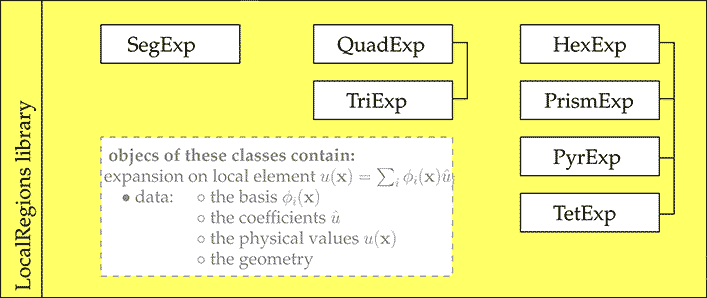
\includegraphics[width=\textwidth]{img/LocalRegions.png}
\caption{Main classes in the LocalRegions library.}
\label{f:library:localregions}
\end{figure}

\section{Collections}
The Collections library contains optimised approaches to performing finite
element operations on multiple elements. Typically, the geometric information is
handled separately to the core reference operator, allowing the reference
operator to be applied to elements stored in contiguous blocks of memory. While
this does not necessarily reduce the operation count, data transfer from
memory to CPU is often substantially reduced and the contiguous storage
structures enable more efficient access, thereby reducing runtime.

\subsection{Structure}
The top-level container is the \texttt{Collection} class, which manages one or
more LocalRegions objects of the same type (shape and basis). The
\texttt{Operator} class generically describes an operation of these elements.
Derived classes from \texttt{Operator} are created for each specific operation
(e.g. BwdTrans, IProductWRTBase) on each element type. A factory pattern is used
to instantiate the correct class using the key triple (shape, operator, impl).
All classes relating to a particular operator are collated in a single .cpp
file.

An example template for a specific \texttt{Operator} class is as follows:
\begin{lstlisting}[style=C++Style]
class [[NAME]] : public Operator
{
    public:
        OPERATOR_CREATE([[NAME]])

        virtual ~[[NAME]]()
        {
        }

        virtual void operator()(
                const Array<OneD, const NekDouble> &input,
                      Array<OneD,       NekDouble> &output,
                      Array<OneD,       NekDouble> &output1,
                      Array<OneD,       NekDouble> &output2,
                      Array<OneD,       NekDouble> &wsp)
        {
            [[IMPLEMENTATION]]
        }

    protected:
        [[MEMBERS]]

    private:
        [[NAME]](
                vector<StdRegions::StdExpansionSharedPtr> pCollExp,
                CoalescedGeomDataSharedPtr                pGeomData)
            : Operator(pCollExp, pGeomData)
        {
            [[INITIALISATION]]
        }
};
\end{lstlisting}
The placeholders in double square brackets should be replaced as follows:
\begin{itemize}
	\item \texttt{[[NAME]]}: The name of the class in the form
	\begin{lstlisting}
	<operation>_<impl>{_<shape>}
	\end{lstlisting}
	where the shape need only be included if the operator is shape-specific.
	\item \texttt{[[MEMBERS]]}: Any member variables necessary to store precomputed
	quantities and ensure computational efficiency.
    \item \texttt{[[IMPLEMENTATION]]}: The code which actually computes the action
    of the operator on the elements in the collection.
	\item \texttt{[[INITIALIZATION]]}: Code to initialize member variables and
	precomputed quantities.
\end{itemize}

\subsection{Instantiation}
Operators are instantiated through the OperatorFactory. Therefore the operator
classes must be registered with the factory during start-up. This is achieved
using static initialisation with either the \texttt{m\_type} or
\texttt{m\_typeArr}. The latter is shown in the following example:
\begin{lstlisting}[style=C++Style]
OperatorKey BwdTrans_StdMat::m_typeArr[] = {
    GetOperatorFactory().RegisterCreatorFunction(
        OperatorKey(eSegment,       eBwdTrans, eStdMat,false),
        BwdTrans_StdMat::create, "BwdTrans_StdMat_Seg"),
    GetOperatorFactory().RegisterCreatorFunction(
        OperatorKey(eTriangle,      eBwdTrans, eStdMat,false),
        BwdTrans_StdMat::create, "BwdTrans_StdMat_Tri"),
    ...
};
\end{lstlisting}
This instructs the factory to use the \texttt{BwdTrans\_StdMat} class for all
shapes when performing a backward transform using the \texttt{StdMat} approach.
In contrast, if the class is shape specific, the non-array member variable would
be initialised, for example:
\begin{lstlisting}[style=C++Style]
OperatorKey BwdTrans_SumFac_Seg::m_type = GetOperatorFactory().
    RegisterCreatorFunction(
        OperatorKey(eSegment, eBwdTrans, eSumFac, false),
        BwdTrans_SumFac_Seg::create, "BwdTrans_SumFac_Seg");
\end{lstlisting}

\section{MultiRegions}
In the MultiRegions library, all classes and routines are related to the
process of assembling a global spectral/hp expansion out of local elemental
contributions are bundled together. The most important entities of this library
are the base class ExpList and its daughter classes. These classes all are the
abstraction of a multi-elemental spectral/hp element expansion. Three different
types of multi-elemental expansions can be distinguished:

\subsection{A collection of local expansions}
This collection is just a list of local expansions, without any coupling between
the expansions on the different elements, and can be formulated as:
\begin{align*}
u^{\delta}(\boldsymbol{x})=\sum_{e=1}^{{N_{\mathrm{el}}}}\sum_{n=0}^{N^{e}_m-1}\hat{u}_n^e\phi_n^e(\boldsymbol{x})
\end{align*}
where
\begin{itemize}
\item ${N_{\mathrm{el}}}$ is the number of elements, 
\item $N^{e}_m$ is the number of local expansion modes within the
element $e$, 
\item $\phi_n^e(\boldsymbol{x})$ is the $n^{th}$ local expansion mode within
the element $e$, 
\item $\hat{u}_n^e$ is the $n^{th}$ local expansion coefficient 
\item within the element $e$.
\end{itemize}

These types of expansion are represented by the classes ExpList0D, ExpList1D,
ExpList2D and ExpList3D, depending on the dimension of the problem (ExpList0D is
used just to deal with boundary conditions for 1D expansions).

\subsection{A multi-elemental discontinuous global expansion}
The expansions are represented by the classes DisContField1D, DisContField2D and
DisContField3D. Objects of these classes should be used when solving partial
differential equations using a discontinuous Galerkin approach. These classes
enforce a coupling between elements and augment the domain with boundary
conditions.

All local elemental expansions are now connected to form a global spectral/hp
representation. This type of global expansion can be defined as:
\begin{align*}
u^{\delta}(\boldsymbol{x})=\sum_{n=0}^{N_{\mathrm{dof}}-1}\hat{u}_n
  \Phi_n(\boldsymbol{x})=\sum_{e=1}^{{N_{\mathrm{el}}}}
  \sum_{n=0}^{N^{e}_m-1}\hat{u}_n^e\phi_n^e(\boldsymbol{x})
\end{align*}
where
\begin{itemize}
\item $N_{\mathrm{dof}}$ refers to the number of global modes, 
\item $\Phi_n(\boldsymbol{x})$ is the $n^{th}$ global
expansion mode, 
\item $\hat{u}_n$ is the $n^{th}$ global expansion coefficient.
\end{itemize}

Typically, a mapping array to relate the global degrees of freedom
$\hat{u}_n$ and local degrees of freedom $\hat{u}_n^e$ is
required to assemble the global expansion out of the local contributions.

In order to solve (second-order) partial differential equations, information
 about the boundary conditions should be incorporated in the expansion. In case
 of a standard Galerkin implementation, the Dirichlet boundary conditions can be
 enforced by lifting a known solution satisfying these conditions, leaving a
 homogeneous Dirichlet problem to be solved. If we denote the unknown solution
 by $u^{\mathcal{H}}(\boldsymbol{x})$ and the known Dirichlet
 boundary conditions by $u^{\mathcal{D}}(\boldsymbol{x})$ then we can
 decompose the solution $u^{\delta}(\boldsymbol{x})$ into the form
\begin{align*}
  u^{\delta}(\boldsymbol{x}_i)=u^{\mathcal{D}}(\boldsymbol{x}_i)+
  u^{\mathcal{H}}(\boldsymbol{x}_i)=\sum_{n=0}^{N^{\mathcal{D}}-1}
  \hat{u}_n^{\mathcal{D}}\Phi_n(\boldsymbol{x}_i)+
  \sum_{n={N^{\mathcal{D}}}}^{N_{\mathrm{dof}}-1}
  \hat{u}_n^{\mathcal{H}}\Phi_n(\boldsymbol{x}_i).
\end{align*}
Implementation-wise, the known solution can be lifted by ordering the known
degrees of freedom $\hat{u}_n^{\mathcal{H}}$ first in the global
solution array $\boldsymbol{\hat{u}}$.


\subsection{A multi-elemental continuous global expansion}
The discontinuous case is supplimented with a global continuity condition. In
this case a $C^0$ continuity condition is imposed across the element
interfaces and the expansion is therefore globally continuous.

This type of global continuous expansion which incorporates the boundary
 conditions are represented by the classes ContField1D, ContField2D and
 ContField3D. Objects of these classes should be used when solving partial
 differential equations using a standard Galerkin approach.


\subsection{Additional classes}
Furthermore, we have two more sets of classes:
\begin{itemize}
\item The class LocalToGlobalBaseMap and its daughter classes:
  LocalToGlobalC0ContMap and LocalToGlobalDGMap.
  
  These classes are an abstraction of the mapping from local to global degrees
  of freedom and contain one or both of the following mapping arrays:
  \begin{itemize}
  \item map $[e][n]$

    This array contains the index of the global degree of freedom corresponding
    to the $n^{th}$ local expansion mode within the $e^{th}$ element.
  \item bmap $[e][n]$
  
    This array contains the index of the global degree of freedom corresponding
    to the $n^{th}$ local boundary mode within the
    $e^{th}$ element.
  \end{itemize}
  Next to the mapping array, these classes also contain routines to assemble the
  global system from the local contributions, and other routines to transform
  between local and global level.
\item The classes GlobalLinSys and GlobalLinSysKey.

  The class GlobalLinSys is an abstraction of the global system matrix
  resulting from the global assembly procedure. Depending of the choice to
  statically condense the global matrix or not, the relevant blocks are stored
  as a member of this class. Given a proper right hand side vector, this class
  also contains a routine to solve the resulting matrix system.
  
  The class GlobalLinSysKey represents a key which uniquely defines a global
  matrix. This key can be used to construct or retrieve the global matrix 
  associated to a certain key.
\end{itemize}

More information about the implementation of connectivity between elements in
Nektar++ can be found [wiki:Connectivity here].

\begin{center}
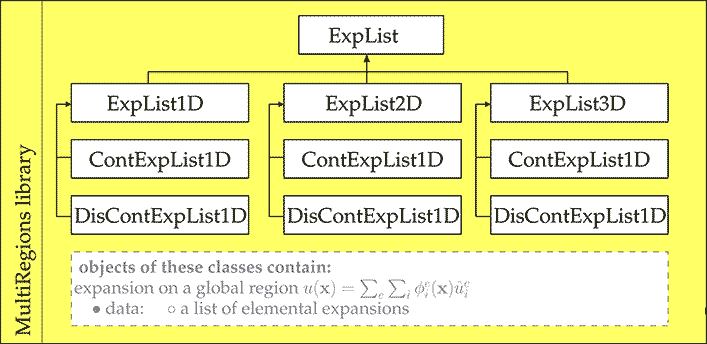
\includegraphics{img/MultiRegions.png}
\end{center}

\subsection{Quasi-3D approach}

The Quasi-3D approach is an extension of the 1D and the 2D spectral/hp element
method. This technique permits to study 3D problems combining the spectral/hp
element method with a spectral method. In the Quasi-3D approach with 1
homogenous direction, the third dimension (z-axis) is expandend with an harmonic
expansion (a Fourier series). In each quadrature point of the Fourier
discretisation we can find a 2D plane discretised with a 2D spectral/hp elements
expasions. In the case with 2 homogeneous directions a plane is discretised with
a 2D Fourier expansion (y-z palne). In each one of the quadrature point of this
harmonic expansion there is a 1D spectral/hp element discretisation. The
homogenous classes derive directly form ExpList, and they are
ExpListHomogeneous1D and ExpListHomogeneous2D. This classes are used to
represent the collections of 2D (or 1D) spectral/hp element problems which are
located in the Fourier expansions quatradure points to create a 3D problem. As
describer above, we can find the find the continuos or discontinuos case,
depending on the spectral/hp element approach. ExpList2DHomogeneous1D and
ExpList1DHomogeneous2D are used to manage boundary conditions. A description of
the Quasi-3D approach usage can be found in Chapter 3 in the User Guide.

\begin{center}
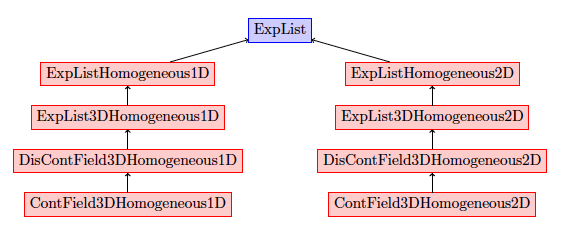
\includegraphics[width=\textwidth]{img/Quasi3d.png}
\end{center}


\section{SolverUtils}

\subsection{Drivers}
Drivers govern the high-level execution of a solver.

\subsubsection{Implementing a new Driver}
To take advantage of the Nektar++ architecture and implement an algorithm 
which will wrap around an existing solver, new drivers can be created. This can
be done in a few steps by using DriverStandard.cpp (and .h) as a template:
\begin{itemize}
\item Create the new files called DriverMyAlgorithm.cpp (and .h)
\item Implement constructor and destructor
\item Provide implementation for \texttt{v\_InitObject} and \texttt{v\_Execute}
as necessary.
\item Register the new driver with the driver factory.
\begin{lstlisting}[style=C++Style]
string DriverMyAlgorithm::className = 
    GetDriverFactory().RegisterCreatorFunction("MyAlgorithm",
                                               DriverMyAlgorithm::create); 
string DriverMyAlgorithm::driverLookupId = 
    LibUtilities::SessionReader::RegisterEnumValue("Driver","MyAlgorithm",0);
\end{lstlisting}
\item Add the new driver to the library. In \inlsh{CMakeLists.txt}, 
DriverMyAlgorithm.cpp must be added in the \inlsh{SOLVER\_UTILS\_SOURCES} 
section and DriverMyAlgorithm.h in the \inlsh{SOLVER\_UTILS\_HEADERS} section.
\end{itemize}


\chapter{Data Structures and Algorithms}


\chapter{Coding Standard}

The purpose of this page is to detail the coding standards of the project which
all contributers are requested to follow.

This page describes the coding style standard for C++. A coding style standard
defines the visual layout of source code. Presenting source code in a uniform
fashion facilitates the use of code by different developers. In addition,
following a standard prevents certain types of coding errors.

All of the items below, unless otherwise noted, are guidelines. They are
recommendations about how to lay out a given block of code. Use common sense and
provide comments to describe any deviation from the standard. Sometimes,
violating a guideline may actually improve readability.

If you are working with code that does not follow the standard, bring the code
up-to-date or follow the existing style. Don’t mix styles.

\section{Code Layout}

The aim here is to maximise readability on all platforms and editors.
\begin{itemize}
\item Code width of 80 characters maximum - hard-wrap longer lines.
\item Use sensible wrapping for long statements in a way which maximises
readability.
\item Do not put multiple statements on the same line.
\item Do not declare multiple variables on the same line.
\item Provide a default value on all variable declarations.
\item Enclose every program block (if, else, for, while, etc) in braces, even if
empty or just a single line.
\item Opening braces (\{) should be on their own line.
\item Braces at same indentation as preceeding statement.
\item One class per .cpp and .h file only, unless nested.
\item Define member functions in the .cpp file in the same order as defined in
the .h file.
\item Templated classes defined and implemented in a single .hpp file.
\item Do not put inline functions in the header file unless the function is
trivial (e.g. accessor, empty destructor), or profiling explicitly suggests to.
\item Inline functions should be declared within the class declaration but
defined outside the class declaration at the bottom of the header file.
\begin{notebox}
Virtual and inline are mutually exclusive. Virtual functions should therefore be
implemented in the .cpp file.
\end{notebox}
\end{itemize}


\section{Space}

Adding an appropriate amount of white space enhances readability. Too much white
space, on the other hand, detracts from that readability.

\begin{itemize}
\item Indent using a four-space tab. Consistent tab spacing is necessary to
maintain formatting. Note that this means when a tab is pressed, four physical spaces are
inserted into the source instead.
\item Put a blank line at the end of a public/protected/private block.
\item Put a blank line at the end of every file.
\item Put a space after every keyword (if, while, for, etc.).
\item Put a space after every comma, unless the comma is at the end of the line.
\item Do not put a space before the opening parenthesis of an argument list to a
function.
\item Declare pointers and references with the * or \& symbol next to the
declarator, not the type; e.g., Object *object. Do not put multiple variables in the same
declaration.
\item Place a space on both sides of a binary operator.
\item Do not use a space to separate a unary operator from its operand.
\item Place open and close braces on their own line. No executable statements
should appear on the line with the brace, but comments are allowed. Indent opening
braces at the same level as the statement above and indent the closing brace at
the same level as the corresponding opening brace.
\item Indent all statements following an open brace by one tab. Developer Studio
puts any specifier terminated with a colon at the same indentation level as the
enclosing brace. Examples of such specifiers include case statements, access
specifiers (public, private, protected), and goto labels. This is not acceptable
and should be manually corrected so that all statements appearing within a block
and delineated by braces are indented.
\item Break a line into multiple lines when it becomes too long to read. Use at
least two tabs to start the new line, so it does not look like the start of a
block.
\item Follow C++ style comments with one space. It is also preferable to
consider any text that follows C++ style comments as a sentence and to begin this text
with a capital letter. This helps to distinguish the line from a continuation of
a previous line; i.e., \inlsh{// This is my comment.} 
\item As a general rule, don’t keep commented out source code in the final
baselined product. Such code leads the reader to believe there was uncertainty 
in the code as it currently exists.
\item Place the \# of a preprocessor directive at column one. An exception is
the use of nested ifdefs where the bodies only contain other preprocessor directives.
Add tabs to enhance readability:
\begin{lstlisting}[style=C++Style]
void foo() { 
    for(int i = 0; i < 10; ++i) 
    { 
#ifdef BAR 
        do_something(); 
#endif
        for_loop_code(); 
    }
}
\end{lstlisting}
\item Use tabular white space if it enhances
readability.
\item Use only one return statement. Structure the code so that only one return
statement is necessary.
\end{itemize}

\section{Naming Conventions}

Keep variable and function names meaningful but concise.
\begin{itemize}
\item Begin variable names with lower-case letter.
\item Begin function names and class names with upper-case letter.
\item All function, class and variable names should be written in CamelCase,
e.g. \inlsh{MyClass, DoFunction() or myVariableName}.
\item All preprocessor definitions written in UPPER\_CASE with words separated
by underscores, e.g. USE\_SPECIFIC\_FEATURE.
\item All member variables prefixed with m\_.
\item All constants prefixed with a k.
\item All function parameters prefixed with a p.
\item All enumerations prefixed with an e.
\item Do not use leading underscores.
\end{itemize}

\section{Namespaces}

The top-level namespace is "Nektar". All code should reside in this namespace or
a sub-space of this.

\begin{itemize}
\item Namespaces correspond to code structure.
\item Namespaces should be kept to a minimum to simplify the interface to their
contents.
\end{itemize}

\section{Documentation}
\begin{itemize}
\item Briefs for classes, functions and types in header files using
\inlsh{///} notation.
\item Full documentation with implementation using \inlsh{/** ... *\/}
notation.
\item Use @ symbol for @class, @param, @returns, etc for ease of identification.
\item Any separate documentation pages not directly associated with a portion of
the code should be in a separate file in /docs/html/doxygen.
\end{itemize}


%\appendix


\backmatter

%%% BIBLIOGRAPHY
%%% -------------------------------------------------------------

\bibliographystyle{plain}
\bibliography{developer-guide}

\printindex

\end{document}
